\section{An�lise L�xica}
Na an�lise l�xica ocorre \ldots
\subsection{Ferramenta JFlex}
A ferramenta JFlex gera analisadores l�xicos em Java a partir da
especifica��o de express�es regulares e trechos de c�digo associados a cada express�o. A especifica��o referida � escrita utilizando a linguaguem JFlex (um clone da linguagem lex), que tem como extens�o .flex.
\begin{figure}[h]
\center
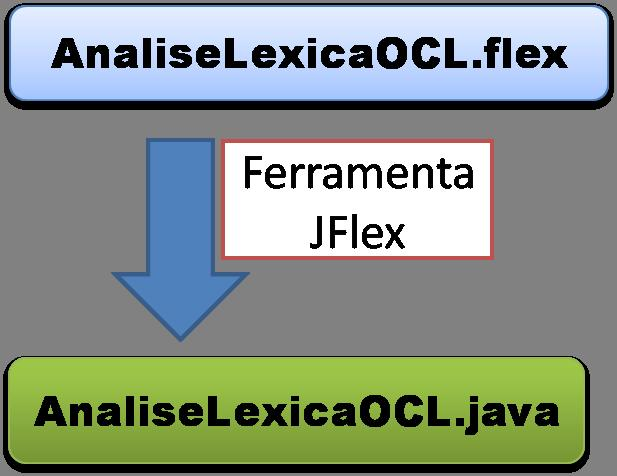
\includegraphics[width=5cm, height=6cm]{ imagens/analiseLexica.jpg }
\caption{ (Esquema - ferramenta JFlex.) }
\label{Imagem representando o uso da ferramenta JFlex.}
\end{figure}